\documentclass[11pt, letter]{article}

% Load packages
\usepackage[style = authoryear, autocite=inline, doi=false,isbn=false,url=false]{biblatex}
\usepackage[margin = 1 in]{geometry}
\usepackage[colorlinks, citecolor = red]{hyperref}
\usepackage{amsmath, amssymb} %essential
\usepackage[long, nodayofweek]{datetime}
\usepackage[]{booktabs}
\usepackage{graphicx}
\usepackage{setspace}
\usepackage{todonotes}
\usepackage[font=small,labelfont=bf]{caption}

% Define symbols
\DeclareRobustCommand{\bbone}{\text{\usefont{U}{bbold}{m}{n}1}}
\DeclareMathOperator{\EX}{\mathbb{E}} % expected value
\DeclareMathOperator{\V}{\mathbb{V}}
\DeclareMathOperator{\Prob}{\mathbb{P}}
\newcommand*{\trans}{^{\mathsf{T}}} %matrix transpose


\begin{document}

% Define Header
\author{Andrew C. Eggers\thanks{Nuffield College and Department of Politics and International Relations, University of Oxford, United Kingdom. \texttt{aeggers@nuffield.ox.ac.uk}}
\and
Tobias Nowacki\thanks{Department of Political Science, Stanford University, CA, United States. \texttt{tnowacki@stanford.edu}}}
\date{\today}
\title{Comparing strategic voting incentives in plurality and instant-runoff elections}

\maketitle

\doublespacing % set line space

\setcounter{section}{3}

% \section{Data and Methods}

% To assess strategic incentives under Plurality and IRV empirically, we rely on data from the  Comparative Study of Electoral Systems (CSES) for a realistic set of preferences and beliefs. The dataset covers 160 surveys from xx different countries, administered shortly before or after an election.\footnote{Two additional cases in the survey, Belarus (20xx) and Lithuania (20xx), are dropped because no respondent specified full preferences over more than two parties.} We focus on the three largest parties (evaluated how?) and label them $A, B, C$ in descending size, respectively. (Some more summary of the data set?)

% We construct the utilities over candidates and beliefs over the electoral outcome directly from the CSES data. For (ordinal) utilities, we take CSES respondents' party like/dislike scores (on a scale from 0 to 10) for parties $A, B, C$. This also implies their preferences over the three parties and determines their voter type (e.g., $abc$). For beliefs about electoral outcomes, we proceed as if respondents were presented with full information about everyone else's ordinal utilities. A "Level-1" voter would then believe everyone else to vote sincerely, such that the expected electoral outcome is a vector of ballot shares, $\bf v_j$.\footnote{I am not sure if we can think of this iterative process as just giving voters successive polls, or whether they need to have specific knowledge about others' utilities (probably not).} A "Level-2" voter would believe that everyone else in the sample is a "Level-1" strategic voter, i.e. votes strategically in expectation of a result with sincere voting. The respondent's belief about the probability distribution of electoral outcomes is then given by

% \begin{equation}
% 	f({\bf v}, s) = \text{Dir}(s \times {\bf v})
% \end{equation}

% where $s$ is a precision parameter (see above). Alternatively, we can think of a Level-2 voter as someone who has just been given a poll of everyone else voting ...(A better way to approach this is probably to start with sincere preferences and then work my way up...)

% \subsection{CSES summary statistics}

% Brief summary of the CSES dataset (countries, cases, three party dominance)

% \emph{Also mentioned in earlier part of Andy's draft -- decide where this belongs}

% \subsection{Weights}

% Our objective is to characterise the general distribution of strategic incentives under Plurality and IRV under realistic distributions of voters. However, the sample of cases in the CSES dataset is not representative. Some countries have more elections surveyed than others, and there is large variance in countries' electorate. To account for these differences, we use two sets of weights:

% \begin{itemize}
% 	\item when calculating individual-level quantities and aggregating at the level of CSES cases, we use the CSES-provided survey weights for each individual observation.
% 	\item when calculating aggregate-level quantities and summarising across CSES cases, we use the following weight for each case:
% 	\begin{equation}
% 		w_j \equiv 
% 	\end{equation}
% \end{itemize}

% \subsection{Iterative Process}

% Having described our approach to constructing preferences and beliefs, next we apply the method provided in Section 2 to calculate strategic incentives and voter's optimal ballot if maximising expected utility under either electoral system. In the first instance, we assume that our voters are Level-1 strategic; that is, they expect everyone else to vote sincerely (or have been given a poll where everyone else declares their sincere vote). Let $v_0$ denote the vector of ballot shares if everyone voted sincerely, and $v_1(v_0)$ if everyone voted strategically while having a belief with an expected outcome at $v_0$. 

% Of course, when constructing respondents' utilities from like-dislike scores, we cannot know if they would report the same quantities had they been accustomed to a different electoral system (e.g., what if the UK had IRV, rather than plurality?). More generally, if I anticipate others voting strategically, too, I will update my expectations accordingly, and my optimal strategic vote may change as a result. This, in turn, will affect everyone else's optimal choice, and so forth. For that reason, we apply the above method iteratively, until the ballot shares converge onto a fixed-point equilibrium (i.e., where, after updating their expectation about others' strategic votes, no-one changes their vote anymore). [Interpreting the 'learning path'].

\section{Results}

\subsection{Expected Benefit, Magnitude, and Prevalence}

We now proceed to present and discuss the results of applying the above method to the CSES data. We show that the expected benefit of strategic voting is higher in Plurality, regardless of how precise beliefs about the expected outcome are, or how strategic voters anticipate others to be. The larger expected benefit is due to both a higher magnitude and a higher prevalence of strategic incentives in Plurality. Decomposing these results further, we find that the probability of a strategic vote being beneficial is (on average) lower in IRV, whereas costs and benefits of strategic voting are more positively correlated in IRV.

For all quantities of interest, we present the average \emph{within} each CSES cases (weighted by individuals' survey weights) as a thin line across all iterations as discussed in Section 3.3.1. We also compute the average \emph{across} all CSES cases (weighted by case's population and number of surveys) and plot it as a thick line.


\begin{figure}[]
	\centering
	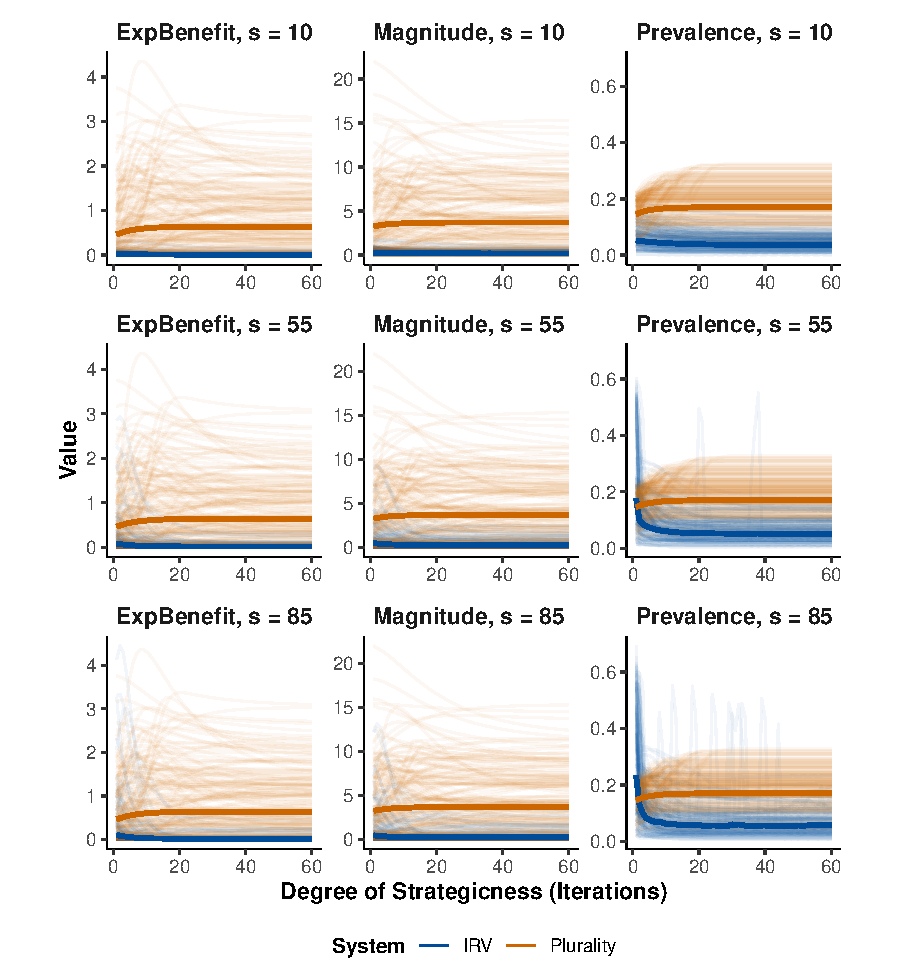
\includegraphics[width = \textwidth]{../output/figures/iterated_complete}
	\caption{Expected benefit, magnitude, and prevalence of strategic voting}
	\label{fig:main_stats}
\end{figure}

Figure~\ref{fig:main_stats} shows the expected benefit, magnitude, and prevalence of strategic voting in both Plurality and IRV. We discuss the expected benefit first, before decomposing the result into magnitude (how much one benefits from the strategic vote) and prevalence (whether one has an incentive to vote strategically at all). Overall, our finding supports the conjecture noted in at the beginning that IRV offers fewer incentives to vote strategically than Plurality.

The expected benefit is higher in Plurality than IRV for all levels of belief precision. Notably, the variance across different CSES cases is also higher in Plurality than in IRV. When beliefs are imprecise ($s = 10$), the expected benefit in Plurality is comparatively lower when voters are expected to vote sincerely (low number of iterations); as voters are expected to become more strategic (high number of iterations), the expected benefit in Plurality reaches approximately the same levels for all levels of precision. Overall, the expected benefit in Plurality is (weakly) increasing in the number of iterations in all three precision settings. 

In IRV, the expected benefit is significantly lower in all circumstances, and there is far less variance across CSES cases. The average expected benefit in IRV does not vary much by level of precision; it remains at very low levels regardless of how precise beliefs are. Note, however, that it is (weakly) decreasing in the number of iterations.

The difference between Plurality and IRV is driven by both the magnitude and the prevalence of strategic incentives in either system. For magnitude (how much does a strategic vote benefit me?), the patterns look very similar to those of the overall expected benefit. The magnitude in Plurality is, on average, higher; it increases in the number of iterations and does so more strongly if beliefs are imprecise. In IRV, the magnitude is unconditionally low for all levels of belief precision, and weakly decreases in the number of iterations.

Finally, the prevalence of strategic voting incentives is somewhat different. We observe similar patterns in Plurality as we did for expected benefit and magnitude: the prevalence is, on average, higher than in IRV, and increases in the number of iterations. However, the difference between the two electoral systems is smaller. In fact, in the case of reasonably precise beliefs and an expectation that everyone else votes sincerely, strategic incentives in IRV are more prevalent. In further difference to the previous two quantities, the average prevalence of strategic incentives in IRV increases notably as precision improves. However, despite the increase in average levels, the prevalence \emph{conditional on the same level of precision} still decreases in IRV as voters are expected to behave more strategically.

In sum, we find that strategic incentives have a higher average expected benefit in Plurality under all circumstances. For the most part, a greater proportion of voters has an incentive to vote strategically in Plurality (prevalence), and if they do, the benefit from doing so (magnitude) is also larger than in IRV. Only when beliefs are precise and everyone else votes sincerely is the prevalence of strategic voting higher in IRV; however, even in these circumstances, the magnitude remains low, still yielding a higher composite expected benefit in Plurality (fewer people having an incentive to vote strategically, but those who do gain more from it).

\subsection{Explaining the Results}

We discuss and explain these findings further.

\subsubsection{Probability of Benefitting from an Insincere Vote}

\emph{Not quite sure if this point predominantly speaks to the magnitude or the prevalence of strategic incentives.}

One of the reasons for the higher magnitude of strategic incentives in Plurality is that the pivotal events that render an insincere vote beneficial have a higher probability of occuring in this electoral system. Recall that in Plurality, an $abc$ voter benefits from casting a $B$ vote if they can resolve a tie for first between $B$ and $C$ ($bc$ pivotal event). In contrast, in IRV, there are multiple pivotal events that can render one's insincere vote beneficial, but they are more complex, impose additional conditions and are therefore (even cumulatively) less likely: for example, an $abc$ voter benefits from voting $BAC$ (putting one's second preference first), if $A$ and $B$ are tied in the first round, and $C$ must beat $A$ in the hypothetical second round, but not must not beat $B$. This event is of a more conditional nature than the tie for first in Plurality. Although there are multiple pivotal events in IRV where a non-sincere vote can be beneficial (the former is just one example for an $ABC$ voter), even their joint probability is, on average, lower than that of the relevant pivotal event in Plurality.

\begin{figure}[!htb]
	\centering
	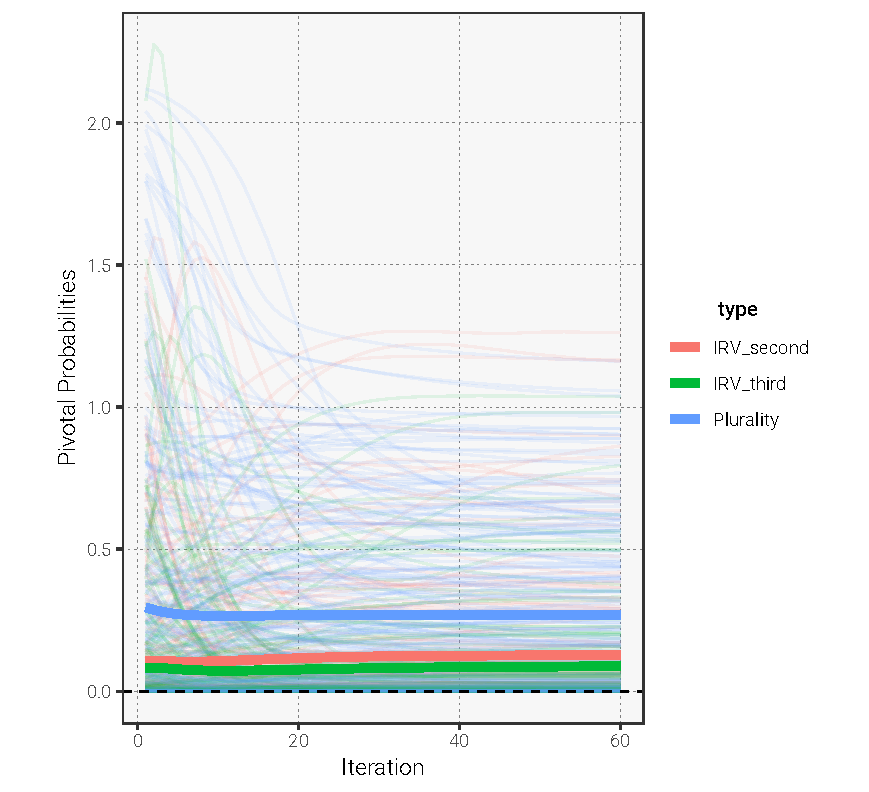
\includegraphics[width = 0.5\textwidth]{../output/figures/conj1}
	\caption{Pivotal probabilities relevant to each strategic vote}
	\label{fig:pivot}
\end{figure}

Figure~\ref{fig:pivot} plots the average probability of a pivotal event under which a non-sincere vote would be beneficial, conditional on precise beliefs ($s = 85$).\footnote{These averages are computed from the likelihood of a pivotal event occuring multiplied with the fraction of voters who would benefit from it --- after all, $abc$ and $cba$ voters' nonsincere votes will be rewarded in different situations.} Each of the categories (IRV second, IRV third, Plurality) refers to the joint average probability that the respective non-sincere vote is beneficial.\footnote{For Plurality, the only relevant non-sincere strategic vote is to vote for one's second preference.} Unlike in the main results (expected benefit), there is a lot more noise between cases here: in some CSES cases, the pivotal probabilities relevant to putting one's third preference first in IRV are higher than those relevant to non-sincere voting in Plurality in other cases. However, the average probability is higher for non-sincere voting in Plurality, followed (by some distance) by one's second preference first in IRV. The average probability of events that reward putting one's third preference first in IRV is the lowest. These averages do not change much as the number of iterations increases.

This result helps to explain why strategic incentives, for the most part, are more prevalent under Plurality: it is more likely that my non-sincere vote has a decisive effect and is rewarded; under IRV, on the other hand, the chance that my non-sincere vote actually affects the outcome in a positive way is much lower.


\subsubsection{Correlation between Benefits and Costs of an Insincere Vote}

The magnitude of strategic incentives is considerably greater in Plurality because the costs and the benefits of insincere voting are negatively correlated: the more I can expect to gain from an insincere vote (the benefit), the less do I have to lose in terms of a possible adverse effect of my nonsincere vote (the cost). Conditional on having any incentive to vote strategically, then, the magnitude is going to be large. In contrast, in IRV, the benefits and costs of insincere voting are positively correlated: the more I can potentially gain from voting insincerely, the greater are the potential adverse effects. Put differently, the risk of my strategic vote `backfiring' is greater in IRV. As a result, the magnitude of strategic voting incentives is comparatively lower.

\begin{figure}[!htb]
	\centering
	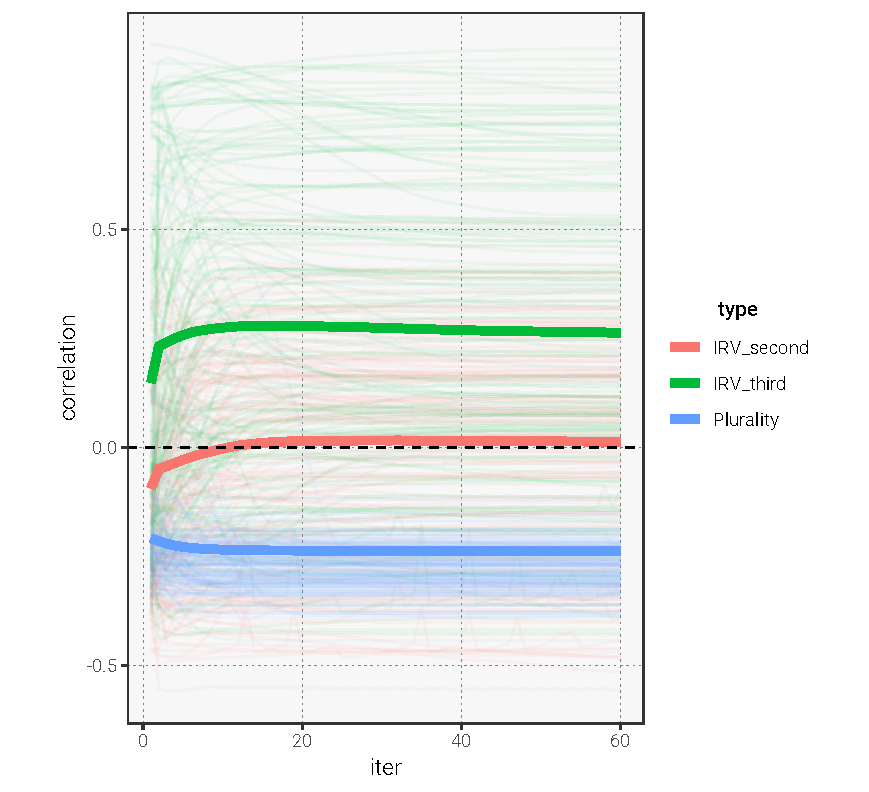
\includegraphics[width = 0.5\textwidth]{../output/figures/conj2}
	\caption{Correlations between benefits and costs for each type of non-sincere vote}
	\label{fig:correl}
\end{figure}

\emph{could decompose risk in prevalence of backfiring events and magnitude of them...}

Figure~\ref{fig:correl} plots the correlation between costs and benefits for each of the non-sincere choices. In Plurality, the two are negatively correlated. This is because what drives strategic incentives is the intention to avoid wasting one's vote. For an $abc$ voter, the closer the expected result is to a pivotal event between $B$ and $C$, the greater is the chance that her vote is wasted, and the more can she benefit from voting for $B$ instead. At the same time, moving closer to this pivotal event also suggests that other pivotal events become less likely: if a tie between $B$ and $C$ becomes more likely, then one between $A$ and $B$ becomes \emph{less} likely (for the most part)\footnote{If we move from one of the vertexes of the distribution, e.g., where $B$ has all votes, towards the centre, then both events can become more likely}. In sum, the risk of a non-sincere vote `backfiring' with severe consequences is low in Plurality. 

In IRV, the correlation is almost zero (for ballots putting one's second choice first) or distinctly positive (for ballots putting one's third choice first). The mechanism is somewhat more complicated (once again). The multitude of pivotal events means that moving closer to a `rewarding' pivotal event often means that nearby, contradictory pivotal events also become more likely. Consequently, the greater the potential benefit from voting insincerely, the greater are also the costs of doing so. This is especially true if putting one's third preference first for strategic reasons: here, the cost is particularly high. If the non-sincere vote backfires, the voter ends up with one's least favourite choice as the winner, which amplifies the cost, even if such an event is not very likely. Overall, nonsincere voting in IRV is riskier: the greater the potential rewards are, the greater are the costs in the adverse case if the vote backfires. This offers an explanation for why the magnitude of strategic incentives is so low in IRV.


\subsubsection{Positive and Negative Feedback}

One other key difference in strategic incentives between the two systems pertains to their behaviour as voters expect overall strategicness to increase (that is, the number of iterations in our algorithm goes up). Both magnitude and prevalence of strategic incentives increases with higher strategicness in Plurality but decreases in IRV. Strategic incentives are complements in Plurality but substitutes in IRV. This difference arises as a result of the nature of strategic voting in the two systems.

In plurality, the main driver to vote insincerely is to avoid wasting one's vote on a trailing candidate. But as a result of a non-sincere vote, the candidate in question ends up trailing even further, which increases the incentive of voters who also have this candidate as first preference to abandon her, too. Thus, we enter a positive feedback loop: abandoning the third-placed candidate triggers others to follow suit, which, in turn, incentivises even more voters to do the same, and so on. This explains why strategic incentives increase in the number of iterations: the more I expect others to behave strategically in Plurality, the more should I expect the trailing candidate to fall behind, and the greater is my incentive abandon her, too. This feedback loop only ends when there is no-one left to abandon the trailing candidate and we settle in a purely Duvergian, two-party equilibrium.

In contrast, negative feedback loops characterise strategic voting incentives in IRV. Recall from Section 3.1. that one of the incentives to vote insincerely in IRV is to abandon a leading candidate in order to avoid wasting one's vote. For example, an $ABC$ voter will vote $CAB$ in order to make sure that $C$ advances to the second round, where their preferred choice, $A$ can beat them. However, doing so decreases A's vote share in favour of C's. If everyone with the same preference ordering did the same, voters run the risk of having too few remaining $A$ voters to beat $C$, and $C$ winning the election.\footnote{Graphically, related to Figure 1, this is the equivalent of `overshooting' the target: the result moves towards $C$'s vertex, but by such a magnitude that it passes through $A$'s winset and settles in $C$'s.} Here, my incentive to engage in this type of strategic voting decreases the more I expect others to act in the same way, lest the insincere vote backfires. This explains why strategic incentives decrease in the number of iterations. It also means that the equilibrium ballot distribution (i.e., the fixed points of the iterative process) do not settle in a Duvergian equilibrum, but rather, all three candidates retain first-preference votes even if everyone votes strategically.

\subsection{Summary}

We show that the average expected benefit of strategic incentives is considerably higher in Plurality than in IRV, regardless of how strategic voters are expected to be or how precise beliefs about the election outcome are. Both prevalence and magnitude are higher in Plurality, with the exception of prevalence in IRV when beliefs are precise and everyone is expected to vote sincerely. We discuss this result with reference to the different nature of strategic voting in either system. In Plurality, pivotal events that benefit a non-sincere vote are more likely than their equivalent in IRV; furthermore, benefits and costs of a non-sincere vote in Plurality are negatively correlated on average. On the other hand, in IRV, we observe that pivotal events that benefit non-sincere voting are less likely, and that the costs and benefits of a non-sincere vote are either uncorrelated (when putting one's second preference first) or positively correlated (when putting one's third preference first). This indicates that opportunities to vote non-sincerely are not only less common in IRV (lower probability of pivotal events), but also that they are riskier and carry a greater cost if they backfire (more positive correlation). Together, these insights help us explain why IRV seems less vulnerable to incentives to vote non-sincerely. Finally, we also discuss the nature of feedback loops in the two systems: Plurality encourages positive feedback loops in strategic incentives, whereas IRV incentivises negative feedback loops. This difference explains why the average expected benefit increases in Plurality as voters become more strategic, but decreases in IRV.



% We now proceed to present and discuss our results. For each quantity of interest, we present the average \emph{within} each CSES case (weighted by the respective survey weights) as a thin line across all iterations. We also compute a weighted average \emph{across} all CSES cases for every iteration, which we plot with a thicker line.\footnote{We can interpret this as a `worldwide' average, if you will...}

% \subsection{Convergence}

% We assume that a fixed proportion $\lambda = 0.05$ of all voters vote strategically in each iteration, and compute strategic incentives and ballot shares as described in Section 2.X.Y. The distribution of ballot shares quickly converges towards a fixed point under both Plurality and IRV in the vast majority of CSES cases. Figure~\ref{fig:convergence} plots the Euclidean distance between the ballot shares from one iteration to the next for every case and iteration under both Plurality and IRV. The average Euclidean distance of ballot shares between the 59th to the 60th iteration is below 0.0014 for Plurality, and below 0.006 for IRV.\footnote{These averages are unweighted -- need to recompile in the future.} Put differently, we can obtain a voting equilibrium, where voters anticipate others' vote choices, and react accordingly, within about 60 iterations from the sincere voting profile.

% \begin{figure}[!tbh]
% 	\centering
% 	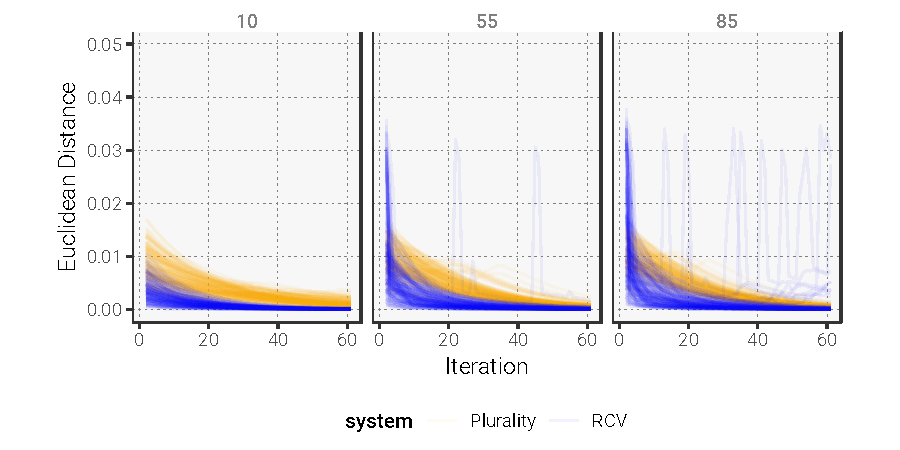
\includegraphics[width = \textwidth]{../output/figures/euclidean}
% 	\caption{Euclidean distance between ballot share vectors from one iteration to another.}
% 	\label{fig:convergence}
% \end{figure}

%  In expectation, convergence towards the fixed point occurs faster under IRV than it does under Plurality. For more precise beliefs ($s \in {55, 85}$), the shift away from the sincere ballot profile in the first few iterations is much larger under IRV than under Plurality; however, faster convergence does not necessarily mean that the fixed point is closer to the original ballot share vector.

%  \begin{figure}[]
% 	\centering
% 	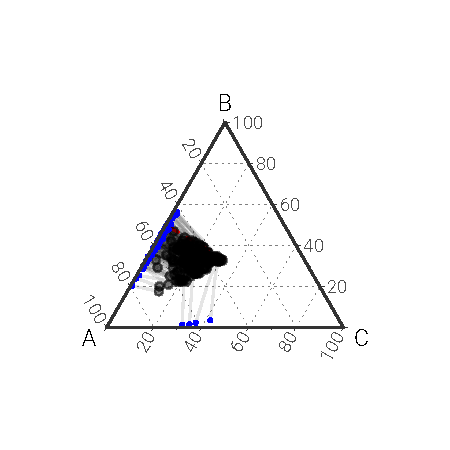
\includegraphics[width = .49\textwidth]{../output/figures/tatonnement_plur}
% 	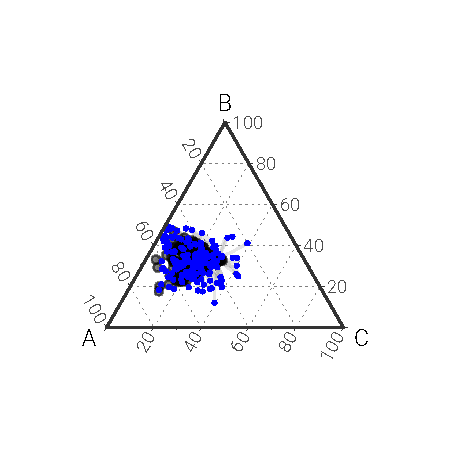
\includegraphics[width = .49\textwidth]{../output/figures/tatonnement_rcv}
% 	\caption{Evolution of ballot share vectors for all CSES cases over iterations, for both Plurality (left) and IRV (right), when $s = 85$. Grey dots indicate the initial ballot share vector before the first iteration; blue dots the ballot share vector after the 60th iteration.}
% 	\label{fig:convergence_paths}
% \end{figure}

%  Figure~\ref{fig:convergence_paths} plots the evolution of ballot shares with increasing iterations under both Plurality and IRV (with ballot shares under IRV aggregated to first preferences). Convergence in plurality is reached when all third-party voters have abandoned their first preference and are voting for the top-two candidates instead, resulting in a Duvergerian two-party equilibrium. There is a handful of cases where the idiosyncratic learning path is such that $B$ is the candidate that ultimately gets abandoned in equilibrium. Under IRV, the fixed point ballot shares are closer to the original (sincere) voting profile and do not yield such extreme results as Plurality (e.g., the third party is not wiped out even if everyone is expected to vote strategically).

%  This result foreshadows a key insight that we discuss further below in Section 5.y: strategic incentives under Plurality are complements (the more I expect other likeminded voters to be strategic, the greater are my own incentives to do so) whereas they are substitutes (my own incentives to vote strategically decrease the more others do so). For now, the main takeaway from the result is that our approach converges on fixed points and we can analyse strategic voting incentives in a situation where the voter anticipates everyone to be sincere, or everyone to be strategic, or any point in between. We also show that, under full convergence and strategic voting, voting behaviour under Plurality converges to a two-party competition, whereas under IRV, first preferences are still cast for all three parties.

% %  As we discussed earlier, strategic incentives under Plurality are characterised by complementarity; this means that with every additional iteration, the incentive for supporters of the third party increases, until all of them have deserted the trailing candidate and the ballot shares are in a Duvergian (two-party) equilibrium.\footnote{We could visualise this by plotting the share of third-party votes when $k = 60$.} In contrast, the substitutability of strategic voting incentives under RCV allows them to reach a fixed point much sooner: as soon as some $ABC$ voters switch to a strategic ($bac$ or $cab$) ballot, the incentive for myself to do equally lessens. Note however, that, for more precise beliefs ($s \in {55, 85}$), the shift away from the sincere ballot profile in the first few iterations is much bigger than under Plurality; quicker convergence does not necessarily mean that the fixed point is closer to the original ballot share vector. This is also related to the substitution / complementary difference: under Plurality, third-party supporters have an incentive to defect towards the top-two that only increases the more other third-party supporters do so. Consequently, the equilibria under Plurality will be such that all third-party supporters will have deserted their first choice and we end up further away from the original distribution of sincere ballots.\footnote{This foreshadows a later result: with sufficiently high precision, the prevalence of strategic voting incentives under IRV will be higher in the first few incentives.}

% % In sum, when applying our iterative strategic voting procedure to all CSES cases, the ballot shares converge more quickly to a fixed point under IRV than under Plurality. Under IRV, these fixed points can occur anywhere in the ballot share space, whereas under Plurality, voters ultimately settle on a two-party Duvergian equilibrium. This is also illustrated by Figure~\ref{fig:convergence_paths}, which maps the ballot share vectors before the first and the 60th iteration for $s = 85$.

% % \emph{(Figure about distance from sincere profile? -- shows nicely that Plurality fixed points are further away from initial ballot shares.)
% % }


% \subsection{Expected Benefit of Strategic Voting}

% Next, we report on the distribution of strategic voting incentives in the form of the expected benefit of doing so in each case.

% \begin{figure}[]
% 	\centering
% 	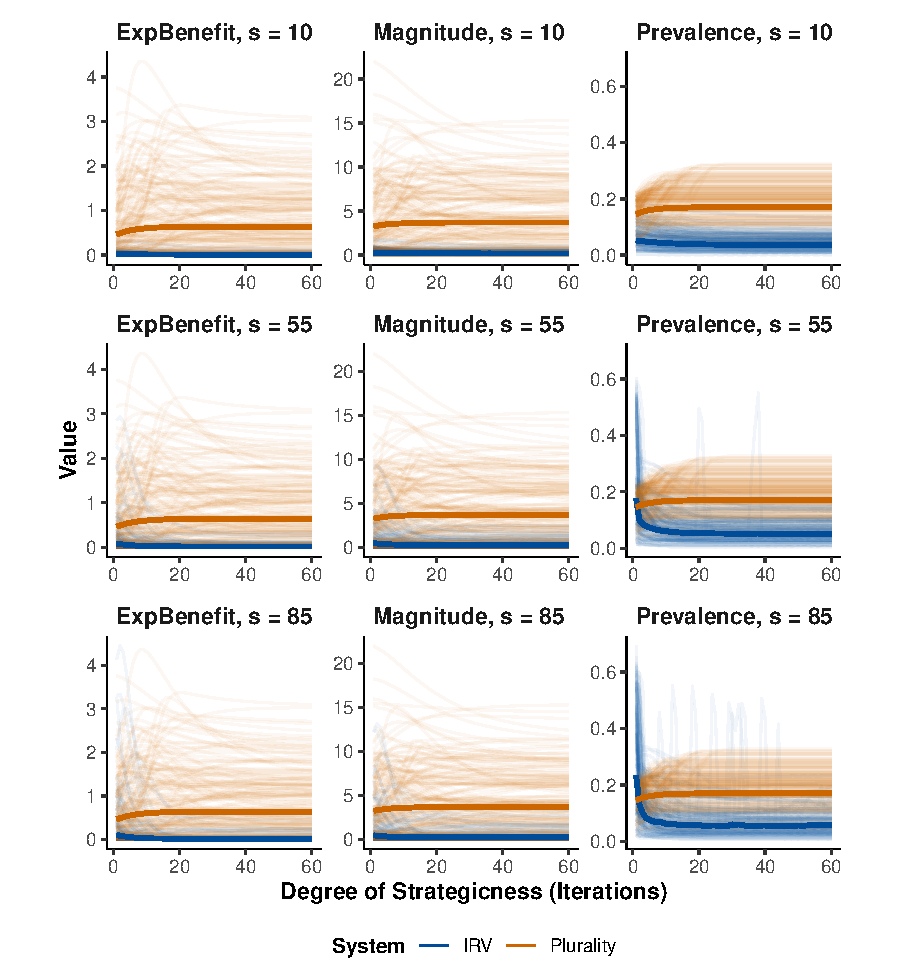
\includegraphics[width = \textwidth]{../output/figures/iterated_complete}
% 	\caption{Main statistics}
% 	\label{fig:main_stats}
% \end{figure}

% Figure~\ref{fig:main_stats} shows the expected benefit of strategic voting (as defined in Section 2.x) for every case at every iteration. 

% We note the following characteristics in the results and will explain and discuss them below. First, the expected benefit is higher for Plurality than for IRV along the entire learning path, independent of the level of precision. This initial finding supports the `folk' conjecture stated in the introduction that IRV offers fewer opportunities for strategic voting. Second, the expected benefit is (weakly) increasing in the number of iterations under Plurality and (weakly) decreasing under IRV. Furthermore, this behaviour becomes more pronounced in Plurality as beliefs decrease in precision. Lastly, the distribution of expected benefits across cases at any given iteration has much higher variance under Plurality than under IRV.

% % What explains the stochastic dominance of Plurality over IRV?\footnote{Not sure if this is the right term since we haven't defined functions her, these are non-parametric estimates.} 
% Strategic voting under Plurality is determined by three main pivotal events --- which two candidates tie for first place. If the third-placed (in expectation) candidate $C$ is performing poorly enough that she has a small chance of tying for first, her supporters will be better off voting for their second preference in case it comes to a tie between the top two candidates, $A$ and $B$. There is little risk of this strategy backfiring: the more likely an $AB$ tie is, the less likely will a $AC$ or $BC$ tie be.\footnote{Strictly speaking this is not true --- if the initial vote share distribution is $(1, 0, 0)$, then all events become more likely as we move out of the vertex.} (In fact, we can assert that strategic voting in Plurality is predominantly driven by those who abandon their first preference that is expected to come third.)

% Contrast this with IRV: because of the two-round nature of the competition, there are more pivotal events to consider, and also greater risks of a strategic vote 'backfiring'. A voter with $abc$ preferences may want to vote strategically by casting a $bac$ ballot; however, doing so carries the risk of backfiring if $A$ and $B$ are tied in either round, or if $A$ and $C$ are tied in the first round.\footnote{In graphical terms, the pivotal events are much closer to one another within the ternary.} (It is much harder for us to characterise \emph{who exactly} votes strategically in IRV.)

% \section{Further Results and Discussion}

% What explains the results reported above? We discuss two key differences in strategic voting between Plurality and IRV. Under Plurality, the predominant incentive comes from abandoning candidates thought to come third; this incentive bears few risks and is generally complementary: the more I expect fellow voters with similar preferences to do so, the larger is my incentive to follow suit. In IRV, incentives to cast a specific ballot bear a greater risk of helping elect a less preferred candidate; (for the most part) they are also strategic substitutes. The more I expect like-minded voters to vote strategically, the lower is my own incentive to do so. Below, we present supplementary evidence for these claims.

% \subsection{Decomposing Expected Benefit}

% We can decompose the Expected Benefit of strategic voting into the magnitude and prevalence of the incentive.\footnote{Recall from Section 2.x that the expected benefit is the product of magnitude and prevalence.} Figure~\ref{fig:main_stats} does exactly this.

% The stochastic dominance of strategic voting incentives in Plurality over IRV is driven by both higher magnitude and (for the most part) prevalence. Similar to the expected benefit, we observe that in both quantities, the statistic (weakly) increases in Plurality, whereas the decrease in expected benefit under IRV seems to be driven by prevalence; the overall magnitude of strategic voting incentives under IRV is very small.

% The fact that both elements of the decomposition share these characteristics can, once again, be explained by referring to the nature of strategic voting under either system. Strategic incentives under Plurality are more prevalent because (a) the pivotal events that make a strategic vote beneficial are more likely to occur under Plurality and (b) the pivotal events that would discourage a strategic vote are less likely to occur under Plurality. The magnitude is higher under plurality because there is little to gain from voting sincerely. The expected third is extremely unlikely to win the election, so voting for her is a wasted vote; the magnitude of the strategic incentive should increase with closeness between the top-two candidates.

% Note that, when expecting everyone else to vote sincerely, prevalence of strategic incentives is actually higher under IRV given high enough precision of beliefs. As mentioned before, the drawback to strategic voting in IRV is the risk of backfiring; the more precise one's beliefs about the expected ballot shares are, the smaller is that risk (since it's less likely that we end up at a `bad' pivotal event). However, even in these cases, the magnitude of these strategic voting incentives is very small: second-round pivotal events in IRV are conditional on the realisation of a particular top-two ranking. Consequently, these events can never be as likely as pivotal events in Plurality, and the magnitude of the benefit is lower.

% \subsection{The Risks of Strategic Voting}

% \begin{figure}[!htb]
% 	\centering
% 	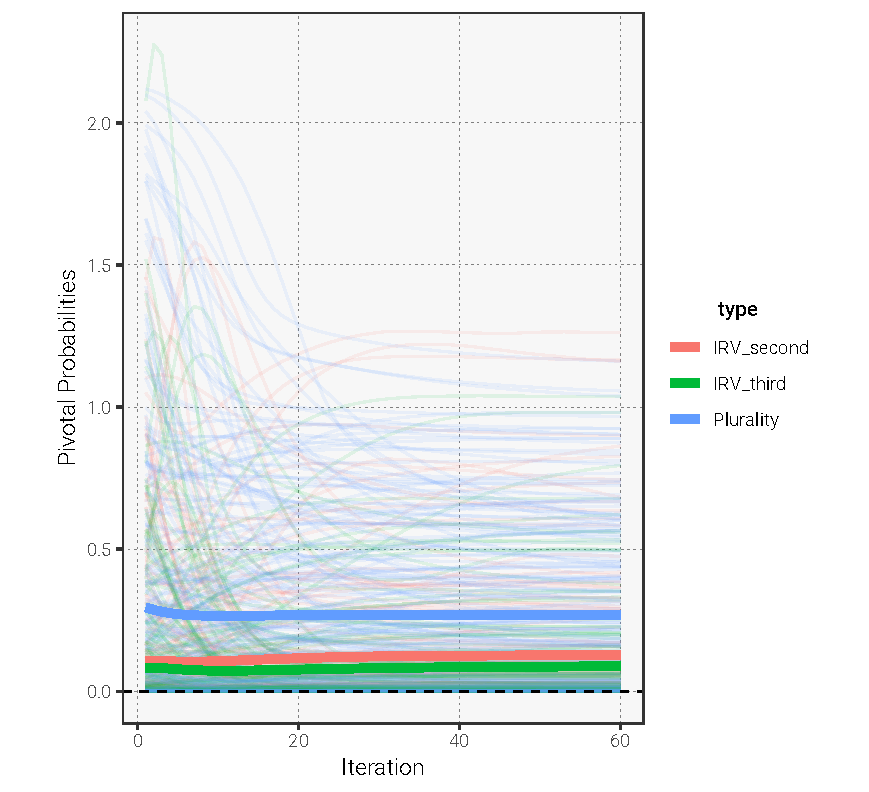
\includegraphics[width = 0.5\textwidth]{../output/figures/conj1}
% 	\caption{Pivotal probabilities relevant to each strategic vote}
% 	\label{fig:pivot}
% \end{figure}

% \emph{Really, this figure should show both probabilities relevant to each strategic vote AND the probabilities where these votes can backfire.}

% We now provide further evidence for the mechanisms that drive the above results. First, we show that the risk of one's strategic vote backfiring is indeed greater under IRV than it is under Plurality. This is in part because the pivotal events under Plurality are more likely, and in part because the benefit of voting strategically at these events is higher / the cost of voting strategically at `discouraging' pivotal events is lower.

% Figure~\ref{fig:pivot} plots the average probability of all pivotal events (at $s = 85$) that render one's strategic vote beneficial. Across all iterations, pivotal events that benefit one's strategic vote under Plurality are more likely than those rendering a vote for one's second or third preference under IRV beneficial. Under plurality, the pivotal event is a tie between the one's second and third preferred candidate for first place. Under IRV, the pivotal events are much more complex and stipulate a second-round tie \emph{conditional on} two particular candidates coming first and second in the first round.

% Next, Figure~\ref{fig:correl} plots the correlation between average costs and benefits of strategic votes. For each type of strategic vote, we multiply the relevant pivotal probability with voters' utility conditional on the pivotal event and their ballot choice. We see that costs and benefits of voting for one's second preference in Plurality are negatively correlated: the higher my gross benefit from voting strategically is, the smaller, on average, will my gross cost be (the less will I have to worry about backfiring). For putting one's second preference first under IRV (IRV-second), the two are largely uncorrelated (but this tells us nothing about their respective magnitude...). Finally, under IRV-third, there is a positive correlation: on average, the higher the benefit, the higher the cost. This underlines the riskiness of putting one's third preference first: in the optimal scenario, it helps, but this also carries the danger of electing one's least favoured candidate if the wrong pivotal event occurs.

% \begin{figure}[!htb]
% 	\centering
% 	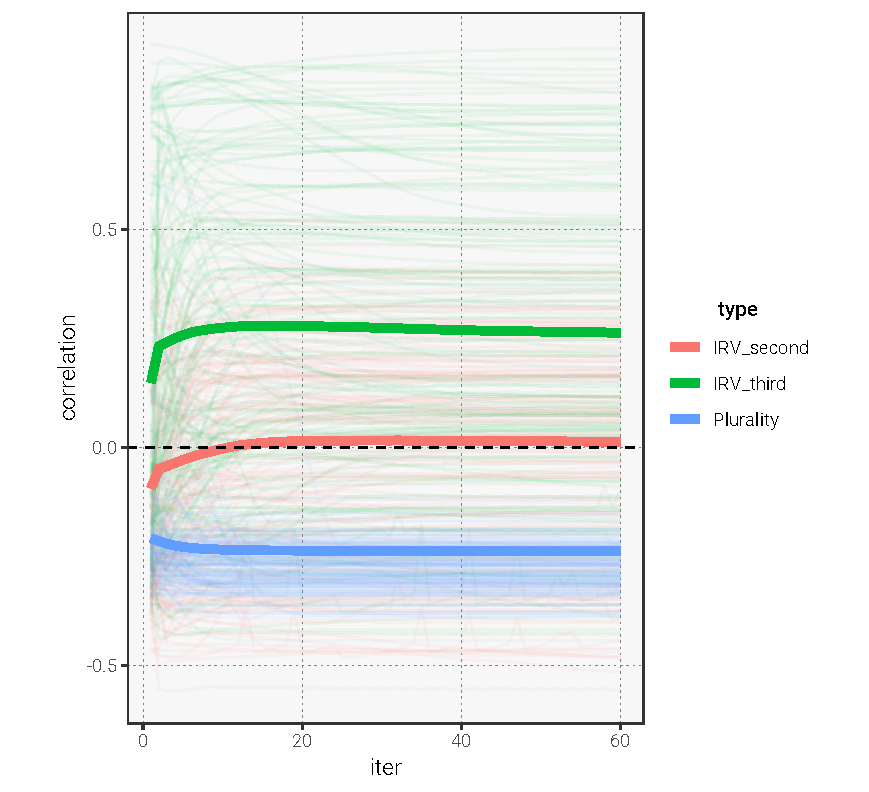
\includegraphics[width = 0.5\textwidth]{../output/figures/conj2}
% 	\caption{Pivotal probabilities relevant to each strategic vote}
% 	\label{fig:correl}
% \end{figure}

% Together, these results highlight the different nature of strategic voting under Plurality and IRV. In the first, strategic incentives are strong if one expects one's first preference to have little chance of winning, and is better off deciding the tie between the top-two candidates instead. There is little risk in this strategy if one's first preference is truly uncompetitive in the race. In IRV, there is a manifold of pivotal events that need to be considered when voting strategically. Here, the chance of one's strategic vote `paying off' is much smaller, and the risk of accidentally electing someone less preferred by voting strategically is much greater. This distinction contributes to the result that strategic voting has a higher expected benefit under Plurality than under IRV.

% % \subsection{Moving Along the Path: Substitution and Complements.}

% % The last part of our discussion seeks to explain the behaviour of strategic incentives along the learning path, that is, as voters' expectations of everyone else's strategicness increase. Recall that, along the path, the expected benefit of strategic voting increases under Plurality, and decreases under IRV.

% % \textit{Main takeaway: discuss expected benefit, magnitude, and prevalence. Show that strategic incentives are, generally speaking, higher under plurality than under IRV. With better information, strategic incentives under IRV become more prevalent, but the benefit of acting on them does not really increase. --> complements and substitudes...}

% % \emph{two things to add: (a) Across all three quantities, plurality increases with higher precision; (b) discuss magnitude?}

% % In this section, we characterise the distribution oxsf strategic incentives along the iterative path. We focus on the prevalence, magnitude and expected benefit of strategic voting under either electoral system. Overall, we find that (a) strategic voting incentives are smaller under IRV than they are under Plurality; (b) as precision of beliefs increases, the prevalence of strategic voting incentives increases under IRV as long as voters believe that the vast majority are voting sincerely (lower number of iterations); it does not change much when voters anticipate widespread levels of strategic voting (higher number of iterations); (c)as the anticipation of other voters' strategicness increases, incentives decrease under IRV but increase under Plurality.

% % We present these results in the form of Figure~\ref{fig:main_stats}, where we plot the weighted average of each quantity within every CSES case conditional on the level of precision (learning path) as a thin line across all iterations. The thicker lines represent the weighted averages aggregated across all CSES cases and are our main point of reference.

% % \begin{figure}[]
% % 	\centering
% % 	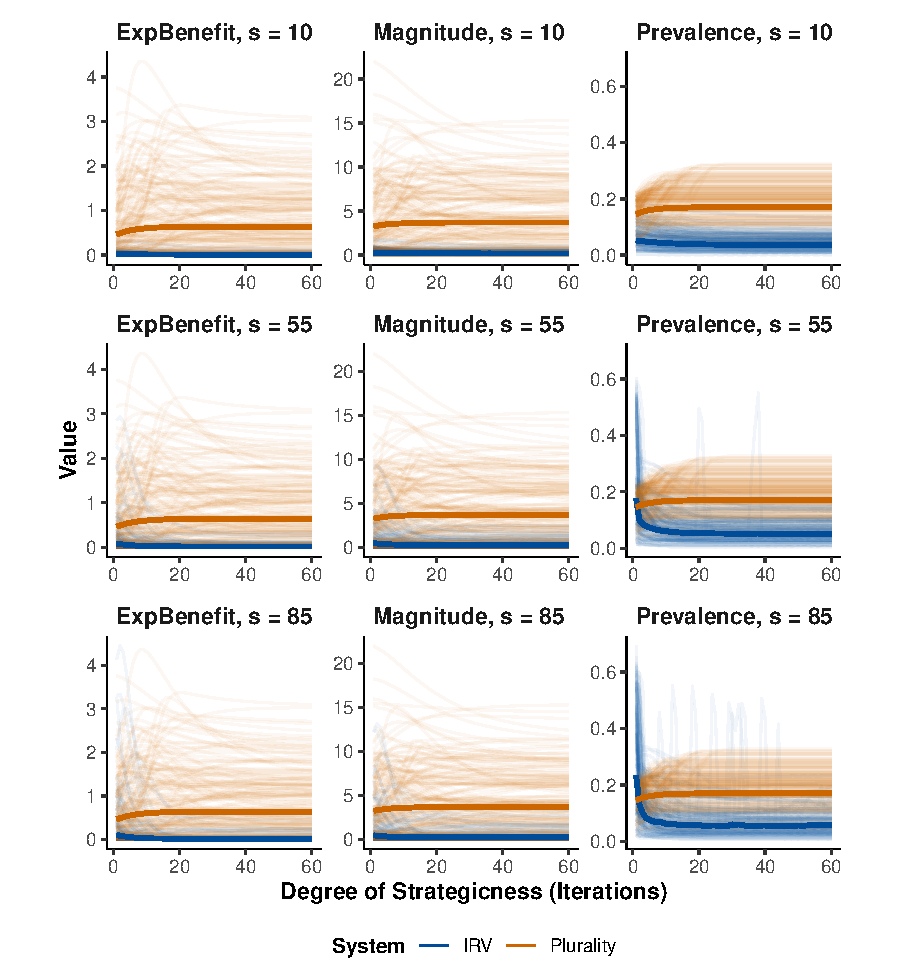
\includegraphics[width = \textwidth]{../output/figures/iterated_complete}
% % 	\caption{Main statistics}
% % 	\label{fig:main_stats}
% % \end{figure}

% % First, we note that the average expected benefit of strategic voting is unconditionally higher under Plurality than under IRV. In line with our previous discussion, strategic voting under Plurality is more straightforward and primarily affects those whose first preference is the likely third-ranked candidate. These voters have a straightforward pivotal event (first/second tie) which, by construction, is much more likely than any other; thus, they face little drawback from voting strategically. Under IRV, on the other hand, voters need to be much more careful as the risk of ending up in a situation where the strategic vote backfires is much greater. This confirms the `folk conjecture' that strategic voting incentives under IRV are less widely distributed.

% % Looking at the prevalence of strategic incentives underlines this intuition: For the most part, incentives are more common in Plurality. However, when the voter anticipates everyone else to vote sincerely (that is, we are at the first iteration) and precision of beliefs is high, the prevalence of strategic voting under IRV is actually quite high (a fifth of the voting population), and slightly higher than that of Plurality. These are the conditions under which a `backfiring' of the strategic vote is least likely. Meanwhile, as we drop to low precision, that incentive becomes less common: with more uncertainty about where the result is going to end up, the risk of casting a `backfiring' strategic ballot becomes greater. For Plurality, the prevalence of strategic voting does not change much across iterations under high precision: with precise beliefs, voters are more certain that their preferred candidate will come last from the onset;\footnote{Unless the second and third are expected to finish very close to one another, of course.} thus already a large proportion of them will desert $C$ from the onset and will continue doing so as more voters become strategic. With more uncertain beliefs, the initial prevalence of strategic incentives under Plurality is lower (as the probability of $C$ tying with either competitor for first place is higher) and increases as strategicness increases and more voters desert $C$ over the course of the iterations.

% % Finally, we note that as voters become more strategic (that is, we move further along the `learning' path and look at a higher number of iterations), the expected benefit of strategic voting increases under Plurality, but decreases under IRV. This refers back to the difference in the nature of the strategic incentives. Under Plurality, strategic incentives are complements: if I am a supporter of the expected third party $C$, my incentive to desert my preferred choice in favour of the top two increases the more other fellow voters do so, too, as the chance of my preferred $C$ winning decreases even further. Consequently, the incentive to vote strategically increases the more I anticipate others doing so, too. Note that this is most prominent in the case with low precision ($s = 10$). Here, the initial prevalence and magnitude are both lower because with higher uncertainty, there is more of a risk of encountering a first-place tie between $C$ and either $A$ or $B$, in which case a non-sincere ballot for $C$-voters would backfire. As strategicness increases, however, the share of $C$ voters decreases and so does the risk of backfiring.\footnote{Graphically, we are travelling from the centre of the vertex towards the A-B line, as $C$ voters desert their most preferred candidate. It is easy to see how such a movement shifts the distribution away from the $AC$ and $BC$ pivotal lines.}

% % In contrast, under IRV, strategic incentives are mostly substitutes: if my fellow like-minded voters already vote strategically, then my additional strategic vote may increase the risk of backfiring and accidentally electing the least-preferred option. As a result, the greater the share of anticipated strategic voters, the lower will my own incentives be.\footnote{Since it is hard to judge the degree of strategicness \emph{ex ante}, this poses a fascinating co-ordination problem in real life...}

% % In sum, the distribution of strategic incentives can be characterised as follows: the average expected benefit of strategic voting is higher in Plurality; with higher precision, the prevalence of strategic incentives improves under either electoral system but more strongly under IRV when voters anticipate everyone else to vote sincerely; finally, as voters' beliefs about others' strategicness increase, the expected benefit increases under Plurality but decreases under IRV.

% % We continue with the remaining quantities of interest to highlight the points made in this discussion further.

% % \subsection{Probability of Pivotal Events}

% % Figure~\ref{fig:pivot} plots the pivotal probabilities for each ballot type as discussed in Subsection~\ref{quants}. Unsurprisingly, the probability is always positive. The average probability of being pivotal with one's strategic vote under Plurality is higher than that of an IRV ballot with one's second preference put first, or that of an IRV ballot with one's third preference put first.

% % \begin{figure}[!htb]
% % 	\centering
% % 	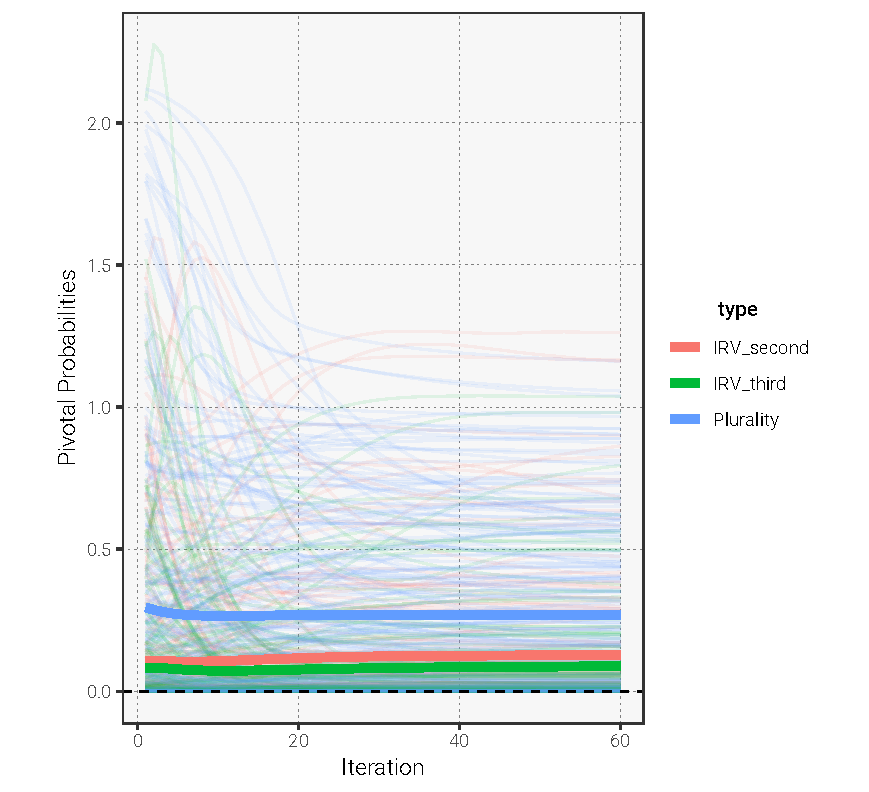
\includegraphics[width = 0.5\textwidth]{../output/figures/conj1}
% % 	\caption{Pivotal probabilities relevant to each strategic vote}
% % 	\label{fig:pivot}
% % \end{figure}

% % (\emph{If we keep the conjectures in the text:}) This provides support for conjecture 1.

% % (\emph{Otherwise:}) Explain / discuss meaning of this along the lines of conjecture 1.

% % \subsection{Expected Costs and Benefits of Strategic Ballots}

% % Finally, we report the average correlation between costs and benefits of strategic ballots in Figure~\ref{fig:correlation}.

% % \begin{figure}[!htb]
% % 	\centering
% % 	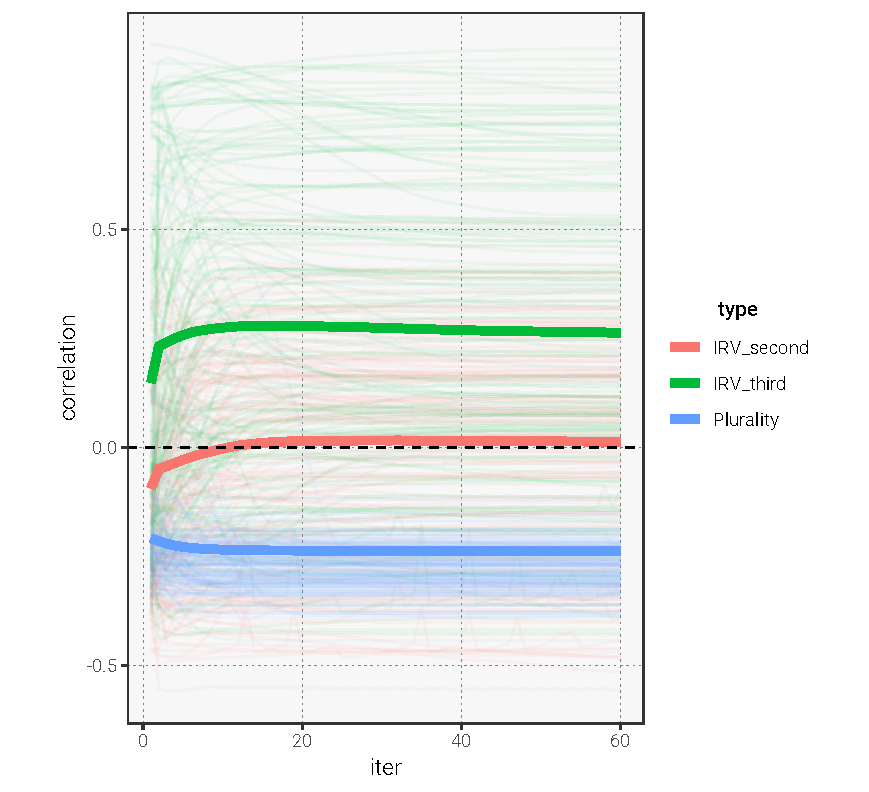
\includegraphics[width = 0.5\textwidth]{../output/figures/conj2}
% % 	\caption{Correlation between costs and benefits of strategic ballots}
% % 	\label{fig:correlation}
% % \end{figure}

% % On average, costs and benefits of a strategic ballot in Plurality (voting for one's second preference, rather than sincerely) are negatively correlated. The result supports conjecture 2. This is in line with our previous discussion: the more likely a tie between $A$ and $B$ is (which favours a strategic vote), the less likely will a tie between $C$ and either of the other candidates be (these are the situations where a strategic ballot would be costly). The interpretation under IRV is somewhat less straightforward and depends on whether the strategic ballot puts one's second or third preference first. In the case of an ``IRV-second'' ballot, costs and benefits are, on average, uncorrelated at higher levels of strategicness. (Why?) Finally, in the case of an ``IRV-third'' ballot, costs and benefits are positively correlated. We can interpret this as an increased risk of ``backfiring'': the rewards of putting one's third preference in first position can be high if the right pivotal event occurs, but equally, so are the risks if one ends up with the worst candidate as the winner (and contributed to electing them). Clearly, backfiring carries a greater 

% % \section{Conclusion}

% \subsection{Substitutes and Complements in Strategic Voting}

% Finally, the distinct evolution of strategic incentives under Plurality and IRV, as well as their different convergence paths, can be explained by the fact that strategic incentives under Plurality are strategic complements, whereas they are strategic substitutes under IRV. As a consequence, when strategic incentives are complementary, the expected benefit rises if more people are doing so; the opposite is true if strategic incentives are substitutes.

% Consider the following case under Plurality. I am a supporter of the expected third party $C$, my incentive to desert my preferred choice in favour of the top two increases the more other fellow voters do so, too, as the chance of my preferred $C$ winning decreases even further. Consequently, the incentive to vote strategically increases the more I anticipate others doing so, too. Note that this is most prominent in the case with low precision ($s = 10$). Here, the initial prevalence and magnitude are both lower because with higher uncertainty, there is more of a risk of encountering a first-place tie between $C$ and either $A$ or $B$, in which case a non-sincere ballot for $C$-voters would backfire. As strategicness increases, however, the share of $C$ voters decreases and so does the risk of backfiring.\footnote{Graphically, we are travelling from the centre of the vertex towards the A-B line, as $C$ voters desert their most preferred candidate. It is easy to see how such a movement shifts the distribution away from the $AC$ and $BC$ pivotal lines.}

% In contrast, in an IRV scenario, if my fellow like-minded voters already vote strategically, then my additional strategic vote may increase the risk of backfiring and accidentally electing the least-preferred option. This is especially dangerous in cases where the strategic incentive would suggest to put one's third preference first. As a result, the greater the share of anticipated strategic voters, the lower will my own incentives be.\footnote{Since it is hard to judge the degree of strategicness \emph{ex ante}, this poses a fascinating co-ordination problem in real life...} To give an example, consider a voter with $abc$ preferences who has an incentive to submit a $cab$ ballot in order to keep $B$ away from the second round. If the voter is, indeed, pivotal in a second-place first-round tie between $B$ and $C$, then this strategic vote would be highly beneficial and return $A$ as the overall winner (if $A$ beats $C$ but not $B$ in the second round). However, if everyone else with the same preference ordering $abc$ does so, such behaviour risks abandoning $A$ to the extent that they either lose to $C$ in the second round or do not even have enough support to advance into the second round. Consequently, the more I expect other voters with the same preference to vote strategically, the smaller should my own incentive to do so be. This illustrates the necessity for co-ordination of strategic voting under IRV and its characterisation of strategic substitutability.

% \subsection{Summary of Results and Discussion}

% We calculated incentives to vote strategically in 160 different elections under both Plurality and IRV for a range of belief precisions and expectations about other voters' strategicness. Overall, we find the following. First, as the voters expect everyone else to vote more strategically, voting behaviour converges to a two-party equilibrium under Plurality, but moves less extremely under IRV. Second, the expected benefit of strategic voting is higher under Plurality compared to IRV. This holds for all levels of precision within our range of analysis and also along the entire `learning path' about other voters' strategicness. Third, both magnitude and prevalence of strategic incentives are greater under Plurality. The only exception is the scenario where beliefs about the election outcome are very precise, and the expectation is that everyone else votes sincerely. In these circumstances, strategic incentives are more widespread under IRV, although they still have a smaller magnitude. Finally, we observe that the expected benefit (and magnitude) of strategic incentives increases in voters' strategicness under Plurality but decreases in voters' strategicness under IRV.

% We discuss these findings and offer an explanation by characterising the different nature of strategic voting in the two electoral systems. Under Plurality, the pivotal events that incentivise strategic voting are more likely; furthermore, the risk of a strategic vote backfiring (causing an election outcome that is worse than if one had voted sincerely) is small, and strategic voting incentives are complementary. Under IRV, pivotal events that reward a strategic vote are comparatively less likely. The risk of `backfiring' is also greater. These two characteristics reduce the prevalence, and magnitude of strategic voting, respectively. Morever, incentives under IRV can be strategic substitutes.

% \section{Conclusion}




\end{document}